\documentclass[a4paper,
fontsize=11pt,
%headings=small,
oneside,
numbers=noperiodatend,
parskip=half-,
bibliography=totoc,
final
]{scrartcl}

\usepackage{synttree}
\usepackage{graphicx}
\setkeys{Gin}{width=.4\textwidth} %default pics size

\graphicspath{{./plots/}}
\usepackage[ngerman]{babel}
\usepackage[T1]{fontenc}
%\usepackage{amsmath}
\usepackage[utf8x]{inputenc}
\usepackage [hyphens]{url}
\usepackage{booktabs} 
\usepackage[left=2.4cm,right=2.4cm,top=2.3cm,bottom=2cm,includeheadfoot]{geometry}
\usepackage{eurosym}
\usepackage{multirow}
\usepackage[ngerman]{varioref}
\setcapindent{1em}
\renewcommand{\labelitemi}{--}
\usepackage{paralist}
\usepackage{pdfpages}
\usepackage{lscape}
\usepackage{float}
\usepackage{acronym}
\usepackage{eurosym}
\usepackage[babel]{csquotes}
\usepackage{longtable,lscape}
\usepackage{mathpazo}
\usepackage[normalem]{ulem} %emphasize weiterhin kursiv
\usepackage[flushmargin,ragged]{footmisc} % left align footnote
\usepackage{ccicons} 

%%%% fancy LIBREAS URL color 
\usepackage{xcolor}
\definecolor{libreas}{RGB}{112,0,0}

\usepackage{listings}

\urlstyle{same}  % don't use monospace font for urls

\usepackage[fleqn]{amsmath}

%adjust fontsize for part

\usepackage{sectsty}
\partfont{\large}

%Das BibTeX-Zeichen mit \BibTeX setzen:
\def\symbol#1{\char #1\relax}
\def\bsl{{\tt\symbol{'134}}}
\def\BibTeX{{\rm B\kern-.05em{\sc i\kern-.025em b}\kern-.08em
    T\kern-.1667em\lower.7ex\hbox{E}\kern-.125emX}}

\usepackage{fancyhdr}
\fancyhf{}
\pagestyle{fancyplain}
\fancyhead[R]{\thepage}

% make sure bookmarks are created eventough sections are not numbered!
% uncommend if sections are numbered (bookmarks created by default)
\makeatletter
\renewcommand\@seccntformat[1]{}
\makeatother


\usepackage{hyperxmp}
\usepackage[colorlinks, linkcolor=black,citecolor=black, urlcolor=libreas,
breaklinks= true,bookmarks=true,bookmarksopen=true]{hyperref}
%URLs hart brechen
\makeatletter 
\g@addto@macro\UrlBreaks{ 
  \do\a\do\b\do\c\do\d\do\e\do\f\do\g\do\h\do\i\do\j 
  \do\k\do\l\do\m\do\n\do\o\do\p\do\q\do\r\do\s\do\t 
  \do\u\do\v\do\w\do\x\do\y\do\z\do\&\do\1\do\2\do\3 
  \do\4\do\5\do\6\do\7\do\8\do\9\do\0} 
% \def\do@url@hyp{\do\-} 
\makeatother 

%meta
%meta

\fancyhead[L]{M. Weil, E. Werner\\ %author
LIBREAS. Library Ideas, 34 (2018). % journal, issue, volume.
\href{http://nbn-resolving.de/}
{}} % urn 
% recommended use
%\href{http://nbn-resolving.de/}{\color{black}{urn:nbn:de...}}
\fancyhead[R]{\thepage} %page number
\fancyfoot[L] {\ccLogo \ccAttribution\ \href{https://creativecommons.org/licenses/by/3.0/}{\color{black}Creative Commons BY 3.0}}  %licence
\fancyfoot[R] {ISSN: 1860-7950}

\title{\LARGE{Studierende, Bücher und Praxis}}% title
\subtitle{Das Projektseminar „Von der Idee zum Buch“ feiert sein 15-jähriges Jubiläum. Ein Interview mit Dr. Petra Hauke}
\author{Martine Weil, Erika Werner} % author

\setcounter{page}{1}

\hypersetup{%
      pdftitle={Studierende, Bücher und Praxis : Das Projektseminar „Von der Idee zum Buch“ feiert sein 15-jähriges Jubiläum. Ein Interview mit Dr. Petra Hauke},
      pdfauthor={Martine Weil, Petra Hauke, Erika Werner},
      pdfcopyright={CC BY 3.0 Unported},
      pdfsubject={LIBREAS. Library Ideas, 34 (2018).},
      pdfkeywords={Bibliothekswissenschaft, Institut für Bibliotheks- und Informationswissenschaft, Humboldt-Universität zu Berlin, Projektseminar, Buchprojekt, Studium},
      pdflicenseurl={https://creativecommons.org/licenses/by/3.0/},
      pdfcontacturl={http://libreas.eu},
      baseurl={http://libreas.eu},
      pdflang={de},
      pdfmetalang={de}
     }



\date{}
\begin{document}

\maketitle
\thispagestyle{fancyplain} 

%abstracts

%body
Kurz vor dem 90-jährigen Jubiläum des Institutes für Bibliotheks- und
Informationswissenschaft der Humboldt-Universität zu Berlin (IBI)
feierte auch das Projektseminar \enquote{Von der Idee zum Buch --
Durchführung eines Publikationsprojektes} sein eigenes Jubiläum. Seit
2002 bietet das IBI den Studierenden die Chance, dieses Projektseminar
zu besuchen. Das Seminar wird einmal pro Jahr angeboten und beschäftigt
sich mit Projektmanagement am Beispiel der Veröffentlichung eines
Sammelbandes zu einem bibliothekswissenschaftlich relevanten Thema.
Dabei lernen die Studierenden in der Praxis die verschiedenen Phasen
eines wissenschaftlichen Publikationsprozesses, von der Themenfindung
bis zur Öffentlichkeitsarbeit. Am Ende jedes Seminars wird ein Buch
veröffentlicht. Bis jetzt sind 14 Bände in Verlagen wie Bock + Herchen
und De Gruyter Saur erschienen. Der 15. Band wird voraussichtlich Ende
2018 erscheinen. Um das 15-jährige Jubiläum dieses erfolgreichen
Projektes zu feiern, haben wir ein Interview mit Dr.~Petra Hauke, seit
15 Jahren Leiterin des Projektseminars, geführt.

\begin{figure}[h!]
\centering
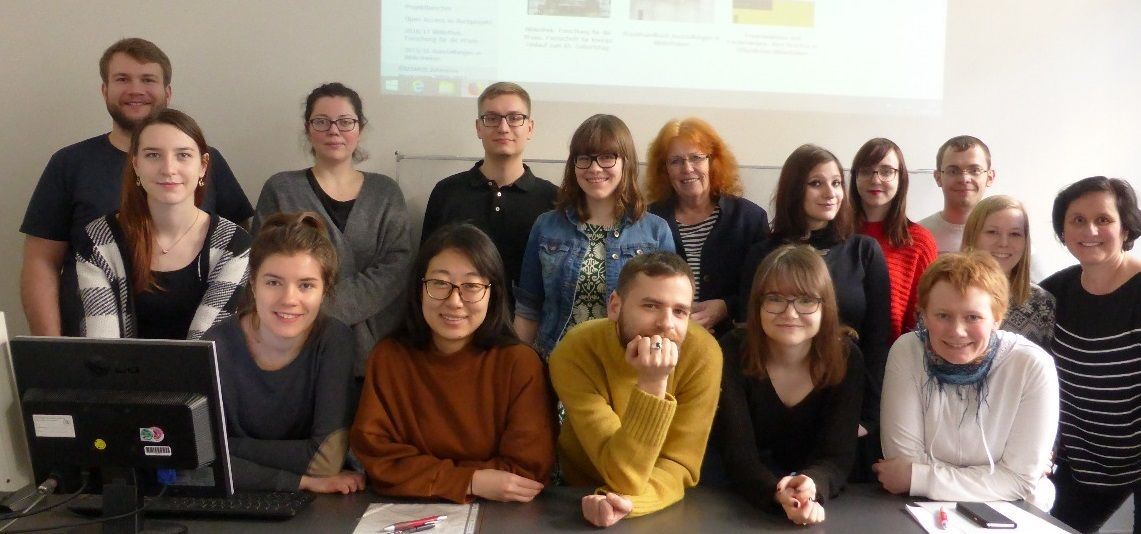
\includegraphics[width=15cm]{img/Bild-01.jpg}
\caption{Dr.~Petra Hauke mit Seminarteilnehmern im Wintersemester
2017/2018 (Fotografie: Valentina Dimitriadu)}
\end{figure}

\pagebreak

\textbf{Martine Weil/Erika Werner: Erfahrung im Projektmanagement ist
heutzutage sehr gefragt. Wie ist die Idee entstanden, ein Seminar zum
Projektmanagement einer Publikation im IBI anzubieten?}

Petra Hauke: In einem Gespräch mit Prof.~Umlauf, der seinerzeit am IBI
lehrte, erzählte ich von einem Lehrauftrag in Hannover zum Thema
Publikationswesen, wo ich mit den Studierenden ein Publikationsprojekt
theoretisch durchgespielt hatte. Zwei Tage später schlug mir
Prof.~Umlauf vor, dies im IBI einmal praktisch anzubieten: \enquote{Von
der Idee zum Buch -- Durchführung eines Publikationsprojektes. Was
halten Sie davon?} So fing es an.

\textbf{MW/EW: Unserer Ansicht nach versucht das Seminar
Bibliothekswissenschaft und Bibliothekspraxis zusammenzubringen. Was
lernen die Studierenden in diesem Kurs?}

PH: Die Studierenden sollten neben den theoretischen Studieninhalten als
künftige Wissenschaftler auch lernen, wie qualitätsvolle, druckreife
Manuskripte aussehen müssen und das nicht nur theoretisch, sondern ganz
praktisch: neben korrekter Rechtschreibung, Zeichensetzung, Grammatik
sowie korrektem Ausdruck und Aufbau auch inhaltliche Logik und
Aussagekraft, schließlich, \emph{last but not least}, korrekte
Zitierungen und Quellennachweise. Das klingt selbstverständlich, ist es
aber nicht, wenn man sich einmal bereits publizierte Arbeiten ansieht,
die zuvor offenbar kein Lektor kritisch geprüft hat.

\textbf{MW/EW: Im Sommersemester 2002 kam das Projektseminar zustande.
Was hat sich seitdem verändert?}

PH: Die Bände sind nicht nur umfangreicher, sondern auch inhaltlich
anspruchsvoller geworden: von \enquote{RAK versus AACR} (2002, 208
Seiten) über \enquote{The Green Library}, ein internationales
IFLA-Projekt (2013, 441 Seiten) bis zu \enquote{Bibliothek. Forschung
für die Praxis: Festschrift für Konrad Umlauf zum 65. Geburtstag} (2017,
730 Seiten).

\textbf{MW/EW: Wie werden die Themen der Bücher ausgewählt?}

PH: Das ist ganz unterschiedlich. Manchmal liegt ein Thema \enquote{in
der Luft}, so wie bei dem ersten Band 2002 nach dem sogenannten
Nikolausbeschluss zum Umstieg auf internationale Formate und Regelwerke,
der eine ziemliche Flut von Diskussionsbeiträgen in Mailinglisten aber
auch Aufsätzen in Fachzeitschriften auslöste. Eine handliche
Publikation, die die verschiedenen Standpunkte zusammenbrachte, schien
damals sinnvoll zu sein. Manchmal ist der Anlass eine Konferenz, deren
mündliche Beiträge durch die Veröffentlichung in einem Sammelband ein
größeres Publikum erreichen sollen. Oder es ergibt sich aus persönlichen
Kontakten beziehungsweise Netzwerkarbeit die Idee der Bündelung
unterschiedlicher Kompetenzen, die einer Publikation zugutekommen
können, wie zum Beispiel bei den Bänden über Bibliotheksbau, die der
Bibliotheksbauexperte Klaus U. Werner nicht nur anregte, sondern als
Mitherausgeber begleitete.

\textbf{MW/EW: Die Veröffentlichung eines Buches ist ein langwieriger
Prozess. Die Veröffentlichung der Beiträge einer Tagung erfolgt in der
Regel erst nach mehreren Jahren.} \textbf{Wie schaffen Sie es, einen
Sammelband so schnell zu veröffentlichen? Wie lange dauert der gesamte
Prozess?}

PH: Ein Semester muss reichen, denn mehr Zeit haben wir nicht zur
Verfügung und jedes Studententeam möchte und soll am Ende sein eigenes
Projekt abgeschlossen in Händen halten können. Das heißt, dass der Kern
der redaktionellen Arbeit an den Beiträgen innerhalb dieses einen
Semesters geleistet wird, mit strengen Terminvorgaben an die beteiligten
Autoren. Mit dem Ende des Semesters sind im Idealfall alle Inhalte
\enquote{ready to print} und gehen an den Verlag. Am Lesen der
Korrekturfahnen beteiligen sich die Studierenden dann nur noch, soweit
es ihre Zeit erlaubt, gegebenenfalls übernehme ich den Part selbst.

\textbf{MW/EW: Was ist der erste Schritt bei der Veröffentlichung eines
Sammelbandes?}

PH: Am Anfang steht die Wahl des Themas. Manchmal wird das erst in der
ersten Sitzung des Semesters beschlossen, woraufhin dann auch erst die
Autorenakquise erfolgt (Freundeskreise und Fördervereine, Praxishandbuch
Ausstellungen in Bibliotheken und so weiter). Bei größeren Projekten
liegen Thema und Autorenbeiträge zu Semesterbeginn bereits als Vorschlag
vor und das Projektteam entscheidet gemeinsam, ob es diesem Vorschlag
folgen oder ein anderes Projekt realisieren möchte.

\textbf{MW/EW: Am Anfang des Kurses haben die Studierenden normalerweise
keine Erfahrung in dem Bereich der Buchveröffentlichung. Vor welchen
Schwierigkeiten steht man, wenn man mit einer Gruppe von Studierenden
ein Buch veröffentlicht?}

PH: Ich spreche ungern von Schwierigkeiten oder Problemen, eher von
Herausforderungen. Die Studierenden gehen, wie wohl die meisten in
dieser Frage Unerfahrenen, davon aus, dass die angesprochenen Autoren
druckfertige Manuskripte einreichen. Dies ist aber eher selten der Fall.
Es gilt also tatsächlich von der Zeichensetzung und Rechtschreibung über
die Grammatik bis hin zur formalen und inhaltlichen Logik und zu
Redundanzen, von den Zitaten (Plagiate!) bis zu den Referenzen
\enquote{auf Punkt und Komma} sehr genau hinzuschauen und gegebenenfalls
zu korrigieren. Besonders sensibel muss bei Stilkorrekturen vorgegangen
werden, immer in Rückkopplung mit den Autoren, die sich aber in der
Regel sehr kooperativ zeigen und uns für unsere Arbeit oft Respekt
zollen.

\textbf{MW/EW: 15 Jahre und 14 veröffentlichte Bücher (das fünfzehnte
Buch wird demnächst erscheinen). Wie viele Studierende haben das
Buchprojekt in all diesen Jahren absolviert?}

PH: Die Teilnehmerzahlen sind unterschiedlich. Sie liegen pro Seminar in
der Regel bei 15 bis 20 Studierenden, wir haben aber auch schon mit nur
5 Studierenden ein Projekt realisiert.

\textbf{MW/EW: Was ist das Wichtigste, das die Studierenden bei dem
Projekt lernen können?}

PH: Die Studierenden lernen vor allem, an ihre eigenen Arbeiten, die sie
künftig zum Beispiel als Hausarbeiten einreichen, entsprechende
Qualitätsmaßstäbe anzulegen. Auch das \enquote{Handwerkszeug}, wie der
Umgang mit Stylesheets, Dokument- und Formatvorlagen oder die
konsequente Anwendung eines bestimmten Zitierstils, kommt ihnen für
eigene künftige Arbeiten zugute. Daneben haben sie die Gelegenheit,
durch den direkten Kontakt mit den Autoren, deren Beiträge sie betreuen,
aber auch mit dem Verlag, Verbindungen für ihr eigenes künftiges
berufliches Netzwerk anzuknüpfen.

\textbf{MW/EW: Die Bücher sind bis jetzt in relevanten Verlagen (Bock +
Herchen, De Gruyter Saur) erschienen. Sind die Verlage normalerweise
offen für solche Projekte?}

PH: Die Wahl des Verlages Bock + Herchen beruhte auf einer zuvor bereits
bestehenden jahrelangen Zusammenarbeit. Bock + Herchen war auch der
erste und einzige Verlag, der, beginnend mit der Festschrift für Walther
Umstätter 2006 als Test, einer zeitgleichen Veröffentlichung der Print-
und der Online-Ausgabe mit Open Access zustimmte. Nachdem die
Buchprojekte sich als erfolgreich erwiesen hatten, zeigten auch andere
Verlage Interesse, jedoch mitunter unter Voraussetzung eines
Druckkostenzuschusses -- den wir nie gezahlt haben -- und in keinem Fall
offen für eine hybride Publikation. Wichtig war uns immer ein namhafter
Fachverlag, sodass unsere Publikation auf dem einschlägigen
\enquote{Markt} auch sichtbar war.

\textbf{MW/EW: Seit 2006 erscheinen die meisten Publikationen des
Buchprojektes in hybrider Form, als Druck- und E-Book-Ausgaben, und man
hat kostenfreien Zugriff auf die meisten Beiträge. Kann man sagen, dass
Open Access zu dem Kurskonzept gehört?}

PH: Ja, Open Access ist Teil des Kurskonzepts (die HU ist
Mit-Unterzeichner der Berliner Erklärung zu Open Access), aber nicht um
jeden Preis. Wir wurden mitunter gefragt, warum wir unsere Bücher
\enquote{nicht einfach ins Netz} stellen. Zum einen steht unser
Qualitätsanspruch einem \enquote{Einfach(!?)-ins-Netz-stellen} entgegen,
zum anderen ist die Wahrnehmung beim Fachpublikum eine andere, wenn ein
profilierter Fachverlag dahintersteht. Da unsere Publikationen nicht
unbedingt von Tagesaktualität abhängen, denken wir, dass es eine
akzeptable Lösung ist, die Bände nach der gesetzlich geregelten
Karenzzeit von 18 Monaten mit Open Access zugänglich zu machen. Der
Verlag unterstützt die Freischaltung, indem er uns das komplette PDF
dafür kostenfrei zur Verfügung stellt. Dieses PDF wird dann von einem
Mitglied des Seminarteams für die Veröffentlichung auf dem edoc-Server
der Humboldt-Universität aufbereitet, dessen Mitarbeiter dann für die
Veröffentlichung und Freischaltung sorgen. Es entstehen also keine
finanziellen Kosten. Es ist schade, dass laut Aussage des Verlages die
Herausgeber anderer Sammelbände von dieser Möglichkeit keinen Gebrauch
machen, andererseits auch verständlich in Anbetracht des technischen
Aufwandes.

\textbf{MW/EW: Ein neues Buch erscheint Ende 2018. Welches Thema wird es
diesmal behandeln? Wie ist das Projekt verlaufen?}

PH: Das Projekt des Wintersemesters 2017/18 basiert auf einer
internationalen Satellitenkonferenz, veranstaltet von ENSULIB, der
Environment, Sustainability and Libraries Special Interest Group der
IFLA, im Vorfeld des Weltbibliothekskongresses 2017 in Polen. Die
Beiträge dieser Konferenz sowie die Beiträge der gemeinsam mit der
Public Libraries Section der IFLA veranstalteten Session in Wroclaw,
dazu einige herausragende Einreichungen zum IFLA Green Library Award
2017 bilden den aktuellen Sammelband. Der Titel lautet \enquote{Going
Green: Implementing Sustainable Strategies in Libraries Around the World
-- Buildings, Management, Programmes and Services}. Die Publikation
wurde vom Professional Committee der IFLA für die Veröffentlichung in
der Reihe \enquote{IFLA Publications} angenommen. Herausgeber sind Petra
Hauke, Madeleine Charney (USA) und Harri Sahavirta (Finland). Eine
besondere Herausforderung stellte die Veröffentlichung in englischer
Sprache dar, zumal, abgesehen von Beiträgen aus den USA und Hongkong,
die eingereichten Beiträge in der Regel von Nicht-Muttersprachlern aus
Brasilien, China, Deutschland, Finnland, Kamerun, Kenia, Portugal,
Schweden, Serbien, Uganda und der Ukraine stammen. Diese mussten auch
sprachlich angepasst werden. Hier haben uns muttersprachliche
Kolleginnen aus der IFLA-Gemeinschaft sehr bereitwillig unterstützt.

\textbf{MW/EW: Das ist schon die zweite Veröffentlichung innerhalb des
Projektseminars, die sich mit Grünen Bibliotheken beschäftigt. Wie
wichtig und aktuell ist das Thema?}

PH: Besonders durch die Annahme der Nachhaltigkeitsziele der UN Agenda
2030 durch die IFLA ist das Thema der \enquote{Grünen Bibliothek} noch
einmal neu und aktuell auf die Tagesordnung gekommen, wie zum Beispiel
auch die Gründung des deutschsprachigen \enquote{Netzwerks Grüne
Bibliothek} im Januar 2018 und die Ankündigung der \enquote{1st
International Conference on Green Libraries: Let's Go Green!} im
November 2018 in Zagreb, Kroatien, zeigen. Auch Veranstaltungen wie der
ungarische und der italienische Bibliothekskongress im März dieses
Jahres in Budapest beziehungsweise Mailand und der Internationale
Bibliothekskongress des österreichischen Bibliotheksverbandes im Mai
2018 sowie der Deutsche Bibliothekartag im Juni 2018 in Berlin haben das
Thema der ökologischen Nachhaltigkeit im Programm.

\textbf{MW/EW: Seit 2005 sind Sie Mitglied bei IFLA-Sektionen und seit
2010 sind Sie aktiv bei der IFLA Environment, Sustainability and
Libraries Special Interest Group (ENSULIB). Das ist der zweite Band, der
in der Reihe \enquote{IFLA Publications} erscheinen wird. Wie läuft die
Zusammenarbeit zwischen dem Projektseminar und der IFLA ab?}

PH: Wenn sich herausstellt, dass wir eine internationale Publikation
anstreben, dann bietet sich an, sie wegen der weltweiten Sichtbarkeit
unter dem \enquote{Schirm} der IFLA zu publizieren anstatt als
Einzelpublikation. Dafür gilt es dann, mindestens eine IFLA-Sektion zu
gewinnen, die die \enquote{Schirmherrschaft} übernimmt. Außerdem müssen
der jeweilige Herausgeber der Reihe sowie das Professional Committee der
IFLA überzeugt werden. Wenn das gelungen ist, ist der Weg für die
Veröffentlichung beim Verlag De Gruyter Saur frei, bei dem die Reihe
erscheint.

\textbf{MW/EW: Die letzte Etappe des Projektseminars ist nicht die
Veröffentlichung des Buches, sondern die Öffentlichkeitsarbeit. Wie wird
dabei vorgegangen? Müssen alle Studierenden Aufgaben aus diesem Bereich
übernehmen?}

PH: Neben der Redaktion der Beiträge gibt es eine ganze Reihe von
Aufgaben, von denen jeweils eine als zusätzliche Aufgabe zu übernehmen
ist. Dazu gehören unter anderem die verschiedenen Aspekte der
Öffentlichkeitsarbeit wie zum Beispiel ein Clip, eine Posterpräsentation
oder ein Vortrag auf dem Deutschen Bibliothekartag, auf der IFLA oder
auf dem internationalen studentischen BOBCATSSS-Symposium, aber auch das
Ansprechen von kompetenten Rezensenten und von einschlägigen
Rezensionsorganen. Besonders die Präsentation des Projektes im Rahmen
eines Kongresses ist für die Studierenden eine in der Regel neue
Erfahrung, die ihren Horizont erweitert und sie ermutigt, künftig auch
ihre eigenen Projekte öffentlich zu präsentieren.

\textbf{MW/EW: Warum ist die Öffentlichkeitsarbeit so wichtig für den
Erfolg eines Projektes? Scheinen die Studierenden gern an dem Prozess
teilzunehmen?}

PH: Ein gutes Produkt erstellt zu haben, ist eine Sache. Aber es auch
\enquote{an den Mann beziehungsweise die Frau zu bringen}, ist eine
andere Sache. Auch wissenschaftliche oder Fachbücher müssen beworben
werden, damit sie ihre Zielgruppe erreichen. Das sehen auch die
Studierenden so, denn ihr Engagement und ihre Kreativität sind gerade in
dieser Hinsicht mitunter bemerkenswert. Es gab schon den Fall, dass eine
Studentin auf sämtliche Weihnachts- und Geburtstagsgeschenke
verzichtete, um ihre Teilnahme an einer IFLA-Konferenz finanzieren zu
können, wo sie das seinerzeitige Buchprojekt mit einem Vortrag und einem
Poster präsentierte.

\textbf{MW/EW: Gibt es Pläne für die Zukunft dieses Seminars?}

PH: Das Seminar wird im Rahmen eines zum jeweiligen Semester neu
erteilten Lehrauftrages angeboten. Im Moment ist ein Auslaufen des
Angebots seitens des IBI nicht erkennbar, und solange die Studierenden
daran interessiert sind und sich immer wieder neue, interessante Themen
finden, stehe ich dafür auch gern noch eine Weile zur Verfügung.

\textbf{MW/EW: Frau Hauke, wir bedanken uns ganz herzlich bei Ihnen.}

PH: Ich bedanke mich bei Ihnen.

Für weitere Informationen über das Projektseminar \enquote{Von der Idee
zum Buch -- Durchführung eines Publikationsprojektes} und die schon
veröffentlichten Bücher besuchen Sie bitte die Webseite des
Buchprojektes unter
\url{https://www.ibi.hu-berlin.de/de/studium/studprojekte/buchidee}.

*Mit Genehmigung der Interviewpartnerin wurden manche Stellen leicht
geändert.

%autor
\begin{center}\rule{0.5\linewidth}{\linethickness}\end{center}

\textbf{Dr.~Petra Hauke} ist seit 2002 Lehrbeauftragte am Institut für
Bibliotheks- und Informationswissenschaft der Humboldt-Universität zu
Berlin (Formalerschließung, Publikationswesen, Auslandsexkursionen).
Ihre Themenschwerpunkte sind Publikationswesen und \enquote{Green Library'}.
Von 2005 bis 2017 war sie Standing-Committee-Mitglied in den
IFLA-Sektionen \enquote{Education and Training'} beziehungsweise \enquote{Library
Theory and Research} und seit 2010 aktiv bei ENSULIB (IFLA Environment,
Sustainability and Libraries Special Interest Group). Sie ist auch eines
der Gründungsmitglieder des \enquote{Netzwerks Grüne Bibliothek --
Interessengemeinschaft für ökologische Nachhaltigkeit}.

\textbf{Martine Weil} studiert Bibliotheks- und Informationswissenschaft
an der Humboldt-Universität zu Berlin.

\textbf{Dr.~Erika Werner} ist Altphilologin und macht zurzeit ein
Zweitstudium der Bibliotheks- und Informationswissenschaft an der
Humboldt-Universität zu Berlin. Die beiden haben das Projektseminar
\enquote{Von der Idee zum Buch -- Durchführung eines Publikationsprojektes} im
Wintersemester 2017/2018 absolviert.

\end{document}
